\subsection{Local characterization of finitely generated projective modules}

THEOREM 1. Let A be a ring and P an A-module. The following properties are equivalent:

\begin{enumerate}
\def\labelenumi{(\alph{enumi})}
\item
  \(\mathbf{P}\) is a finitely generated projective module.
\item
  \(\mathbf{P}\) is a finitely presented module and, for every maximal ideal \(\mathfrak{m}\) of \(\mathbf{A}\) , \(\mathbf{P}_{\mathfrak{m}}\) is a free \(\mathbf{A}_{\mathfrak{m}}\) -module.
\item
  P is a finitely generated module, for all \(p \in \text{Spec}(A)\) , the \(A_{p}\) -module \(P_{p}\) is free and, if we denote its rank by \(r_{p}\) , the function \(p \mapsto r_{p}\) is locally constant in the topological space \(\text{Spec}(A)\) (that is, every point of \(\text{Spec}(A)\) admits a neighbourhood in which this function is constant).
\item
  There exists a finite family \((f_{i})_{i\in \mathbf{I}}\) of elements of \(\mathbf{A}\) , generating the ideal \(\mathbf{A}\) , such that, for all \(i\in \mathbf{I}\) , the \(\mathbf{A}_{f_i}\) -module \(\mathbf{P}_{f_i}\) is free with finite rank.
\item
  For every maximal ideal m of A, there exists \(f \in A - m\) such that \(P_{f}\) is a free \(A_{f}\) -module of finite rank.
\end{enumerate}

We show the theorem by proving the following scheme of implications

\pandocbounded{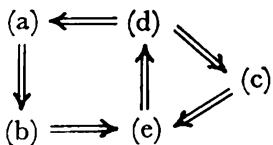
\includegraphics[keepaspectratio]{images/part001_f1dfd2f3.jpg}}

\begin{enumerate}
\def\labelenumi{(\alph{enumi})}
\item
  \(\Rightarrow\) (b): We know that a finitely generated projective module is finitely presented (Chapter I, § 2, no. 8, Lemma 8 (iii)); if P is a projective A-module, \(P_{m} = P \otimes_{A} A_{m}\) is a projective \(A_{m}\) -module (Algebra, Chapter II, § 5, no. 1, Corollary to Proposition 4); finally, as \(A_{m}\) is a local ring, every finitely presented projective \(A_{m}\) -module is free (§ 3, no. 2, Corollary to Proposition 5).
\item
  \(\Rightarrow\) (e): This follows from the Corollary to Proposition 2 of no. 1.
\item
  \(\Rightarrow\) (e): Let \(m\) be a maximal ideal of \(A\) ; write \(r_m = n\) and let \((x_i)_{1 \leqslant i \leqslant n}\) be a basis of \(P_m\) . We can assume that the \(x_i\) are canonical images of elements \(p_i \in P\) ( \(1 \leqslant i \leqslant n\) ) to within multiplication by an invertible element of \(A_m\) . Let \((e_i)_{1 \leqslant i \leqslant n}\) be the canonical basis of \(A^n\) and \(u: A^n \to P\) the homomorphism such that \(u(e_i) = p_i\) for \(1 \leqslant i \leqslant n\) . As \(P\) is finitely generated, it follows from Proposition 2 of no. 1 that there exists \(f \in A - m\) such that \(u_f\) is surjective. We conclude that \(u_{fg}\) is also surjective for all \(g \in A - m\) and by hypothesis there exists \(g \in A - m\) such that \(r_p = n\) for \(p \in X_g\) . Then, replacing \(f\) by \(fg\) , we may assume that \(r_p = n\) for all \(p \in X_f\) . Then \(u_p: A_p^n \to P_p\) is a surjective homomorphism and \(P_p\) and \(A_p\) are both free \(A_p\) -modules of the same rank; hence (§ 3, no. 2, Corollary to Proposition 6) \(u_p\) is bijective for all \(p \in X_f\) . Let \(p'\) be a prime ideal of \(A_f\) and let \(p\) be its inverse image in \(A\) under the canonical mapping; if \((A_f^n)_{p'}\) and \((P_f)_{p'}\) are identified with \(A_p^n\) and \(P_p\) under the canonical isomorphisms, \((u_f)_{p'}\) is identified with \(u_p\) and is consequently bijective. We conclude that \(u_f\) is bijective (§ 3, no. 3, Theorem 1), which establishes (e).
\item
  \(\Rightarrow\) (d): Let E be the set of \(f\in A\) such that \(\mathbf{P}_f\) is a finitely generated free \(\mathbf{A}_f\) -module. The hypothesis implies that E is contained in no maximal ideal of A, hence E generates the ideal A and there therefore exist a finite family \((f_{i})_{1 \leqslant i \leqslant n}\) of elements of E and \(a_{i} \in \mathbf{A}\) ( \(1 \leqslant i \leqslant n\) ) such that \(1 = \sum_{i=1}^{n} a_{i} f_{i}\) ; whence (d).
\item
  \(\Rightarrow\) (c): It follows from no. 1, Corollary to Proposition 3 that P is finitely generated. On the other hand, for every prime ideal p of A, there exists an index \(i\) such that \(\mathfrak{p} \in \mathrm{X}_{f_i}\) ; if \(\mathfrak{p}' = \mathfrak{p}_{f_i}\) , then \(\mathrm{P}_{\mathfrak{p}} = (\mathrm{P}_{f_i})_{\mathfrak{p}'}\) (§ 2, no. 5, Proposition
\end{enumerate}

\begin{enumerate}
\def\labelenumi{\arabic{enumi})}
\setcounter{enumi}{9}
\tightlist
\item
  and hence by hypothesis \(\mathbf{P}_{\mathfrak{p}}\) is free and of the same rank as \(\mathbf{P}_{f_i}\) , which proves (c).
\end{enumerate}

\begin{enumerate}
\def\labelenumi{(\alph{enumi})}
\setcounter{enumi}{3}
\tightlist
\item
  \(\Rightarrow\) (a): Consider the ring \(\mathbf{B} = \prod_{i\in I}\mathbf{A}_{f_i}\) and the B-module
\end{enumerate}

\[
\mathbf {M} = \prod_ {i \in I} \mathrm{P} _ {f _ {i}} = \mathrm{P} \otimes_ {\mathbf {A}} \mathrm{B}.
\]

For every index \(i\), there exists a free \(\mathbf{A}_{f_i}\)-module \(\mathbf{L}_i\) such that \(\mathbf{P}_{f_i}\) is a direct factor of \(\mathbf{L}_i\) and it may be assumed that all the \(\mathbf{L}_i\) have the same rank; then

\(L = \prod_{i \in I} L_i\) is a free B-module of which M is a direct factor, in other words M is a finitely generated projective B-module. As B is a faithfully flat A-module (no. 1, Proposition 3), we conclude that P is a finitely generated projective A-module (Chapter I, § 3, no. 6, Proposition 12).

COROLLARY 1. Suppose that the equivalent properties of the statement of Theorem 1 hold. Let \(m\) be an integer \(>0\) such that, for every family \((x_{i})_{1\leqslant i\leqslant m}\) of elements of \(\mathbf{P}\) , there exists a family \((a_{i})_{1\leqslant i\leqslant m}\) of elements of \(\mathbf{A}\) , which are not all divisors of zero and for which \(\sum_{i=1}^{m} a_i x_i = 0\) . Then, for all \(p \in \operatorname{Spec}(A)\) , \(r_p \leqslant m\) .

Let \(p\) be a prime ideal of \(A\); set \(r = r_p\), and let \((y_j)_{1 \leqslant j \leqslant r}\) be a basis of the free \(\mathbf{A}_{p}\)-module \(\mathbf{P}_{p}\). There exist elements \(x_j\) (\(1 \leqslant j \leqslant r\)) of \(\mathbf{P}\) and \(s \in A - p\) such that \(y_j = x_j / s\) for all \(j\). Then for every family \((a_j)_{1 \leqslant j \leqslant r}\) of elements of \(A\) such that \(\sum_{j=1}^{r} a_j x_j = 0\) , \(\sum_{j=1}^{r} (a_j / 1) y_j = 0\) in \(P_p\) , whence \(a_j / 1 = 0\) for \(1 \leqslant j \leqslant r\) . As \(A - p\) does not contain 0, this shows that the \(a_j\) are all divisors of zero in \(A\) ( \(\S 2\) , no. 1, Remark 3), hence of necessity \(r \leqslant m\) .

COROLLARY 2. Every finitely presented flat module is projective.\par

If P is a finitely presented flat A-module and m a maximal ideal of A, the \(A_{m}\) -module \(P_{m}\) is flat (§3, no. 4, Proposition 13) and finitely presented (§2, no. 4) and hence free (§3, no. 2, Corollary 2 to Proposition 5), Condition (b) of Theorem 1 therefore holds.

Remarks

\begin{enumerate}
\def\labelenumi{(\arabic{enumi})}
\item
  There exist finitely generated flat modules which are not projective (Exercise 7).
\item
  Corollary 2 to Theorem 1 extends to modules over non-commutative rings (Chapter I, § 2, Exercise 15).
\end{enumerate}
% semantic-fragments: legacy-input-seam
\relax{}
